\chapter{Machine-Screened Failure Analysis}
\label{chap:machine-results}

The benchmark results in \Cref{chap:benchmark-results} establish final performance but do not identify the stage at which correctness appears or disappears. This chapter uses the frozen Mistral screening snapshot to analyse all 8,000 MAS item-configurations and 26,873 intermediate stage outputs. The results provide breadth and failure localisation; they are screening evidence rather than human-validated prevalence estimates.

\section{Semantic discovery, oracle coverage, and aggregation regret}

The full-trace Mistral screen indicates that independent-candidate architectures frequently make the correct answer available before the final decision. Aggregation regret, defined in \Cref{eq:regret} as candidate-oracle accuracy minus final semantic accuracy, is the quantity that separates the two. For frozen MuSiQue at 1,000 tokens, Debate has final semantic accuracy 0.720 and candidate-oracle accuracy 0.845, giving aggregation regret of 0.125. Ensemble has final accuracy 0.660 and oracle accuracy 0.960, a regret of 0.300. Parallel Roles is more extreme: final accuracy 0.600 versus oracle accuracy 0.915, a regret of 0.315. These gaps are too large to describe as candidate-generation failure alone.

\begin{figure}[htbp]
  \centering
  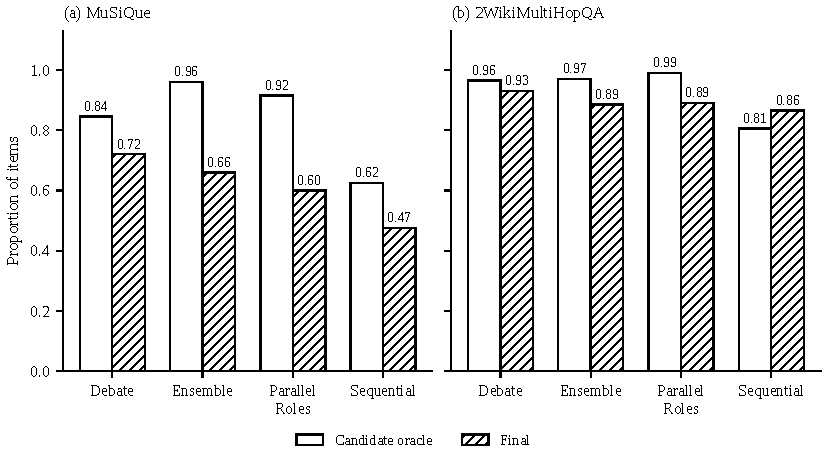
\includegraphics[width=0.94\textwidth]{figures/semantic_oracle_final.pdf}
  \caption[Candidate-oracle and final semantic accuracy]{Machine-screened candidate-oracle and final semantic accuracy for the frozen model at the 1,000-token budget. Higher oracle than final accuracy indicates that a correct candidate was available but not selected. Subtask Parallel is omitted because its worker outputs are partial findings rather than full-answer candidates.}
  \label{fig:oracle-final}
\end{figure}

\Cref{fig:oracle-final} shows that the gap is dataset dependent. On frozen 2Wiki at 1,000 tokens, Debate's final accuracy is 0.930 and its oracle accuracy 0.965, a regret of only 0.035. Ensemble and Parallel Roles still show positive regret, at 0.085 and 0.100. Easier questions allow both candidates and aggregators to be more reliable; on MuSiQue, candidate diversity increases without a comparable increase in final decision quality.

The semantic diversity statistic supports this interpretation. Frozen MuSiQue Parallel Roles has diversity rate 0.650 and a mean of four distinct candidate texts, while its final semantic accuracy is only 0.600. Ensemble has mean 3.835 distinct candidates and final accuracy 0.660. Diversity is therefore a resource, not an outcome. It creates selection opportunities and selection risk simultaneously.

Sequential behaves differently. In this machine-screened breadth analysis, its candidate oracle is an any-correct summary over the worker outputs, whereas the human final-boundary audit uses only the last worker as its source. These quantities must not be conflated. On frozen MuSiQue at 1,000 tokens, the worker-set oracle is 0.625 and final accuracy is 0.475. On 2Wiki, final accuracy exceeds the worker-set oracle (0.865 versus 0.805 at 1,000), producing negative regret. This is consistent with an aggregator synthesising partial or implicit findings into a correct final response. Negative regret does not imply perfect preservation; it indicates that the final stage sometimes creates answer-equivalent content not credited in any individual worker output.

\section{Machine-screened terminal-failure attribution}

Across 8,000 MAS item-configurations, the rule-based screen classifies 5,876 trajectories as finally correct under the machine label and 2,124 as terminal failures (26.6\%). Of all configurations, 946 (11.8\%) end wrong with no correct intermediate Discovery detected; the implementation assigns these directly to the initial/proposal category rather than locating a first causal error step. Among the remaining terminal failures, 73 (0.9\%) are assigned to Debate revision, 75 (0.9\%) to the Sequential worker chain, 173 (2.2\%) to the Debate final picker, and 857 (10.7\%) to final aggregation. The last category includes Ensemble, Parallel Roles, Sequential, and Subtask Parallel and is the largest pooled assigned boundary class.

\begin{table}[htbp]
  \centering
  \caption[Machine-screened terminal-failure attribution]{Mutually exclusive rule-based terminal-failure classes as count (percentage of the architecture's 1,600 item-configurations). ``No detected discovery'' means that the final output is wrong and no correct intermediate Discovery was detected; it is not a stepwise localisation of the first causal error. The final row uses all 8,000 MAS item-configurations. These are descriptive screening estimates, not human-validated prevalence.}
  \label{tab:first-error}
  \scriptsize
  \setlength{\tabcolsep}{2.5pt}
  \begin{tabular}{@{}lrrrrrr@{}}
    \toprule
    System & \shortstack{No detected\\discovery} & Revision & Worker chain & Picker & Aggregator & \shortstack{Any terminal\\failure} \\
    \midrule
    Debate & 77 (4.8) & 73 (4.6) & 0 (0.0) & 173 (10.8) & 0 (0.0) & 323 (20.2) \\
    Ensemble & 66 (4.1) & 0 (0.0) & 0 (0.0) & 0 (0.0) & 316 (19.8) & 382 (23.9) \\
    Parallel Roles & 77 (4.8) & 0 (0.0) & 0 (0.0) & 0 (0.0) & 336 (21.0) & 413 (25.8) \\
    Sequential & 376 (23.5) & 0 (0.0) & 75 (4.7) & 0 (0.0) & 94 (5.9) & 545 (34.1) \\
    Subtask Parallel & 350 (21.9) & 0 (0.0) & 0 (0.0) & 0 (0.0) & 111 (6.9) & 461 (28.8) \\
    \midrule
    All & 946 (11.8) & 73 (0.9) & 75 (0.9) & 173 (2.2) & 857 (10.7) & 2,124 (26.6) \\
    \bottomrule
  \end{tabular}
\end{table}

These rates make the architecture denominators explicit: for example, Sequential's 94 aggregator losses are 5.9\% of its 1,600 screened item-configurations, whereas Ensemble's 316 aggregation failures are 19.8\%. They should not be compared with a supposed SAS ``aggregation rate'': SAS has no picker or aggregator, and the same Mistral pre-final-Discovery-to-final-Endorsement screen has not yet been completed for its 1,600 traces.

Within Debate, the screen counts 278 harmful proposal-to-revision flips and 169 beneficial flips. A targeted human sensitivity audit exactly confirmed 13 of 24 resolved sampled harmful flips and 11 of 25 beneficial flips. A descriptive projection retained the direction harmful greater than beneficial, but the modest confirmation rates mean the raw full-trace counts cannot be presented as exact semantic totals. Similarly, the machine screen identifies 142 Sequential items where the worker chain ends wrong after earlier discovery and 94 in which the aggregator loses a correct last-worker answer. Only 8 of 25 sampled machine-labelled Sequential \ctow{} transitions were exactly confirmed in the targeted audit, mainly because the judge over-called source correctness.

These results locate picker and aggregator boundaries as high-value targets, but they do not substitute for the final human audit.

\section{Resource associations and truncation}

Within matched design strata, observations above the median wall time have lower odds of discovery (adjusted OR 0.657, 95\% CI $[0.574,0.753]$) and higher odds of dropping the answer after discovery (OR 1.768, $[1.529,2.044]$). Above-median realised thinking tokens show the same direction: OR 0.529 ($[0.456,0.613]$) for discovery and OR 2.679 ($[2.153,3.334]$) for post-discovery drop.

\begin{figure}[htbp]
  \centering
  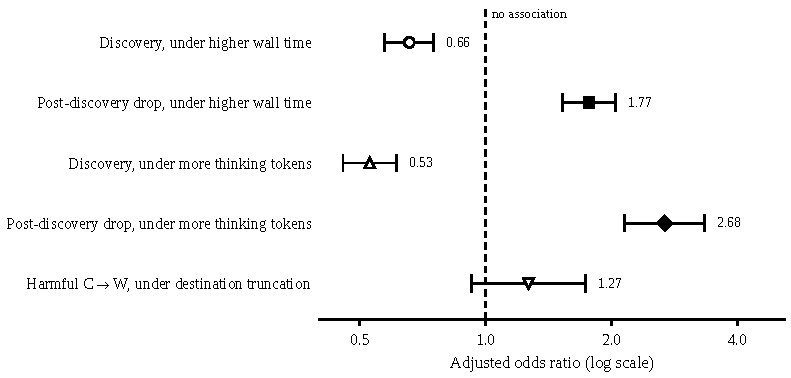
\includegraphics[width=0.90\textwidth]{figures/resource_associations.pdf}
  \caption[Resource exposure and semantic outcomes]{Adjusted observational odds ratios for resource exposure and semantic outcomes. Values below one favour the unexposed group for the named outcome; intervals are 95\% confidence intervals. These associations are not causal effects.}
  \label{fig:resources}
\end{figure}

These results do not mean that fewer tokens causally improve reasoning. Difficult or unstable items may elicit longer trajectories, and repeated unsuccessful revisions may consume both time and tokens. They show that realised compute is not a valid proxy for productive reasoning in this experiment.

Destination-stage truncation has OR 1.268 for a \ctow{} transition conditional on a correct machine-labelled source, with 95\% CI $[0.926,1.736]$ and $p=0.139$. The interval includes one, so the data do not establish a truncation effect. Furthermore, the targeted human audit found lower exact machine--human transition agreement for truncated destinations (0.412) than for non-truncated destinations (0.604). Truncation is thus both a plausible failure mechanism and a condition under which the automated judge is less dependable; the present evidence is insufficient to make a causal claim.

\section{Why human validation is required}

The broad screen supplies scale, but its most consequential errors occur in the transition-enriched cases required for mechanism claims. A single source-stage error can change an item's transition class, and the machine counts above therefore cannot be interpreted as exact failure prevalence. \Cref{chap:human-results} first evaluates audit reliability and then reports the population-weighted transition estimates derived from human labels.
